\PassOptionsToPackage{quiet}{xeCJK}
\documentclass[withoutpreface,bwprint]{format}
\usepackage{placeins}
\usepackage{needspace}











%%%%%%%%%%%%%%%%%%%%%%%%%%%%%%%%%%%%%%%%%%%%%%%%%%%%%%%%%%%%%
%% 正文
\begin{document}

% 将每张长表作为一个整体排版，避免表格跨页拆分。
\setcounter{LTchunksize}{10000}

%  报名信息表（封面标题上方）
%   下列 tihao / baominghao / group 等赋值宏由软件「队伍信息」自动填充（injectTeamInfo），
%   表格单元格用 mcm@tokens@ 取值显示，无需手改。
%   tihao = 题号；group = 组别（封面「所属类别」单元格用）
\tihao{}
\baominghao{}
\group{}
\schoolname{}
\membera{}
\memberb{}
\memberc{}
\supervisor{}




% 标题
{\centering\zihao{3}\bfseries 基于滚动时域优化与情景分析的微网购电储能模型\par}

\setcounter{page}{1}

\thispagestyle{plain}

\begin{abstract}

本文主要研究了微网购电与储能问题。光伏出力与负载需求的偏差会增加微网补购电量，储能与合同调整则为降低费用提供了空间。本文以购电费用最小为目标，建立含储能的线性规划模型，依次研究确定性调度、紧急购电、合同调整和波动电价。\par\medskip

针对问题一，我们将负载与光伏预测换算为10分钟时段电量，以能量守恒、储电量递推与边界、充放电功率上限及首末储电量相等为约束，在此基础上建立了确定性线性规划模型，并采用HiGHS求解。
求解结果如下：

\textbf{全天购电量为59482.70~kWh，购电费为35126.95元，较无储能方案节省26.90\%。}\par\medskip

针对问题二，我们根据周同期负载和近期光伏数据预测净负荷并校正偏差，按误差分位数增加采购保护量，结合末端储电价值确定日前合同。
在此基础上建立了含紧急购电惩罚的滚动计划模型。
求解结果如下：

执行时根据实际余缺充放电，储能不足的部分由紧急购电补足。\textbf{统计期内购电费为13790848.69元，其中紧急购电费为468467.64元，占3.40\%。}\par\medskip

针对问题三，我们将当时已发布的光伏预报细化为10分钟曲线，与历史统计预测按误差加权组合；由线性规划生成备选合同，再按历史误差情景中的净增益均值决定是否调整。
在此基础上建立了基于线性规划与情景净增益的滚动优化模型。
求解结果如下：

\textbf{统计期内购电费为13298484.49元，较问题二方案节省3.57\%，紧急购电量下降43.43\%，1002次机会中调整265次。}日前组合光伏预测的MAE为127.90~kW，较历史预测降低14.83\%。\par\medskip

针对问题四，我们用前一周同时段电价与历史偏差中位数预测价格，分别求解合同不可调整与可调整两类场景。可调整场景按同一历史日期配对净负荷误差和对数价格误差，比较备选合同的情景净增益均值。
在此基础上建立了价格误差情景驱动的购电储能优化模型。
求解结果如下：

\textbf{两类方案购电费分别为14526595.92元和14018361.30元，较固定电价分别上升5.34\%和5.41\%；可调整方案较不可调整方案节省3.50\%。}\par\medskip

本文的创新主要体现在预测信息利用与合同调整评价的结合。针对单一预测难以及时反映光伏变化、合同调整难以兼顾当期费用与跨日储电价值的问题，我们采用分时发布预报与历史预测的误差加权组合，依据历史净负荷误差分时设置采购保护量，并在相同决策点、储电状态和历史误差路径下配对比较调整与保持合同，将调整费用及末端储电短缺机会成本纳入净增益评价。\textbf{该方法提升了预测信息的利用效率，增强了合同修正对供需变化的适应性，并使费用评价兼顾当前结算与跨日储能价值，可用于微网日前购电、日内合同修正及虚拟电厂储能协同调度。}

\keywords{微网经济调度；线性规划；滚动时域优化；组合预测；经验分位数；情景分析}

\end{abstract}

% 正文采用略宽行距，改善连续段落的可读性。
\renewcommand{\baselinestretch}{1.15}\normalsize
\section{模型假设}

为简化问题，本文做出以下假设：

假设1：典型日的电价、小区负载与光伏发电功率在每个10分钟时段内保持不变，且逐日完全重复，即问题一中的优化是在完全信息下进行的确定性决策。

假设2：将题目中的“充放电效率为90\%”按充、放电两个环节的单程效率理解，即储能设备的充电效率与放电效率均恒为0.9且不随储电量与功率变化；充放电过程不存在自放电损耗，储电量在0:00至24:00之间始终处于1200至10800 kWh的允许区间内。

假设3：光伏发电与小区负载的预测误差具有短期平稳性，可用最近若干个完整日的实测误差样本刻画其分布，调度中心仅使用决策时已完成时段的观测与已经发布的预报。

假设4：微网与外网之间的功率交换不受联络线容量限制，计划与调整仅在题定时刻提交，剩余供电缺口允许紧急采购；不向外网售电。问题四的未来价格视为未知，决策用历史价格预测，实际结算用附件4实现价。

\section{符号说明}
各变量采用10分钟时段能量口径，功率乘以$\Delta t$后进入优化模型。$E_t$表示第$t$时段开始时的储电量，$E_{t+1}$表示该时段结束时的储电量；上标$(d)$标识日期，下标$t$标识日内时段，预测量加帽号表示。
\begingroup\small
\begin{longtable}{>{\centering\arraybackslash}p{0.23\textwidth}p{0.52\textwidth}>{\centering\arraybackslash}p{0.15\textwidth}}
\caption{主要符号及量纲}\label{tab:符号说明}\\
\toprule 符号 & 含义 & 单位或取值\\\midrule\endfirsthead
\caption{主要符号及量纲（续）}\\\toprule 符号 & 含义 & 单位或取值\\\midrule\endhead
\bottomrule\endfoot
$d,t,T$ & 日期索引、日内时段索引及每日时段数$T=144$ & $t=0,\ldots,143$\\
$\Delta t$ & 单个时段时长 & $1/6$ h\\
$s,t_s,\mathcal F_s^{(d)}$ & 预报发布序号、对应起始时段及决策信息集 & $s=0,1,2,3$\\
$L_t,V_t,N_t$ & 负载、光伏及净负荷电量，$N_t=L_t-V_t$ & kWh\\
$\hat L_t,\hat V_t,\hat N_t$ & 负载、光伏及净负荷预测电量 & kWh\\
$Y_{s,t},\omega_t,b^O_{s,h}$ & 细化官方预报、融合权重及官方预报偏差 & kWh、无量纲、kWh\\
$p_t,\hat p_t$ & 实现电价与决策时预测电价 & 元/kWh\\
$q_t,a_t,h_t$ & 原计划、生效合同及紧急购电量 & kWh\\
$\Delta_t^+,\Delta_t^-$ & 生效合同相对原计划的上调与下调电量 & kWh\\
$c_t,d_t,w_t$ & 充电、放电及未消纳供电量 & kWh\\
$E_t,E_0,E_H$ & 时段初始、窗口初始及窗口末端储电量 & kWh\\
$E_{\min},E_{\max}$ & 储电量运行下限与上限 & 1200、10800 kWh\\
$P_{\max},\bar Q$ & 充放电功率上限及单时段电量上限 & 5000 kW、$5000/6$ kWh\\
$\eta_c,\eta_d$ & 充电效率与放电效率 & 均为0.9\\
$\alpha,Q_\alpha,\mathcal R_{d,h}$ & 保护分位水平、经验分位数及历史误差集 & 无量纲、kWh、集合\\
$B_t^{\mathrm{lo}},B_t^{\mathrm{hi}}$ & 净负荷0.70与0.90分位数边界 & kWh\\
$\lambda,\mathcal L$ & 合同混合系数及候选方案集合 & $\{0,0.5,1\}$、集合\\
$\varsigma,\mathcal P$ & 历史误差情景索引及情景集合 & $|\mathcal P|\le14$\\
$G_\varsigma,\hat G_\varsigma$ & 原始费用节省及末端储电修正后的净增益 & 元\\
$D_\varsigma,\kappa$ & 末端储电短缺及其评价系数 & kWh、元/kWh\\
$\varepsilon_C,r$ & 均值净增益门槛；$r$仅用于含最坏损失限制的实验对照 & 均为5元\\
$\nu,W$ & 优化目标末端储电价值系数与历史误差档案长度 & 0.45元/kWh、28日\\
$W_{\mathrm{obs}}$ & 问题二及四-2的同小时保护观测数 & 28个观测\\
$\beta$ & 日内预测偏差衰减系数 & 0.90\\
$\zeta_t,\rho$ & 对数价格预测误差与压力测试放大系数 & 无量纲\\
$P_t,Q_t$ & 原始功率记录与折算后的时段电量 & kW、kWh\\
$Y^{(h)},u_t,z_{s,t}$ & 逐小时预报节点、相对发布时刻与预报偏差 & kW、h、kWh\\
$\mathrm{MAE},\mathrm{RMSE},\mathrm{WAPE}$ & 预测误差评价指标 & kW、kW、\%\\
$\bm{x},\bm{c},A_{\mathrm{eq}},A_{\mathrm{ub}}$ & 线性规划变量、目标系数及等式/不等式约束矩阵 & 按模型维度\\
$C,F$ & 实际结算费用与含末端价值的优化目标 & 元\\
\end{longtable}\endgroup
局部使用的$h$为小时编号，紧急购电量始终写为$h_t$；日期索引$d$与放电变量$d_t$通过上下标区分。问题一以$F$表示典型日实际费用，年度模型以$C$表示账单、以$F$表示优化评价值。


% ════════════════════════════════════════════
% 四个问题的分析、建模与求解章节
% ════════════════════════════════════════════
% 每问由独立的一级标题和四个二级标题组成：分析、数据预处理（按需）、建模、求解。
% 图表来自 figures/ 与 tables/；正式数值依据 results/official/ 和 results/diagnostics/。
% ════════════════════════════════════════════
\section{问题一的分析、建模和求解}

\subsection{问题一的分析}

问题一的主要矛盾是，在电价、负载和光伏预测均已知的条件下，协调储能充放电与外网购电时序，以降低典型日购电费用。由于输入信息完全确定，本问可作为后续不确定性调度模型的基准。

\subsection{问题一的建模}

\subsubsection{数据预处理}

附件1以10分钟为采样间隔。令$\Delta t=1/6$ h，将负载与光伏功率统一折算为时段电量
\begin{equation}\label{eq:src1}
L_t=P_{\mathrm{load},t}\Delta t,\qquad V_t=P_{\mathrm{pv},t}\Delta t,\qquad t=0,1,\ldots,143 .
\end{equation}
原始00:10记录对应自然日00:00--00:10，24:00记录对应23:50--24:00；正文按自然日区间报告，结果模板保留附件5的原有行标签，二者的对应关系见支撑材料时间映射表。

\subsubsection{目标函数}

设$a_t,c_t,d_t,w_t$分别为第$t$时段外网购电量、储能充电量、储能放电量和未消纳电量（kWh），$E_t$为储电量。前置参数为$T=144$、$\Delta t=1/6$ h、$E_0=E_{144}=6000$ kWh、$E_{\min}=1200$ kWh、$E_{\max}=10800$ kWh、$P_{\max}=5000$ kW及$\eta_c=\eta_d=0.9$。以全天购电费最小为目标。

\textbf{我们建立以下典型日确定性购电模型：}
\begin{align}
\min\quad &F=\sum_{t=0}^{143}p_ta_t,\label{eq:src5}
\end{align}

\subsubsection{约束条件}
\begin{align}
\mathrm{s.t.}\quad
&a_t+V_t+d_t=L_t+c_t+w_t,\label{eq:src6}\\
&
 E_{t+1}=E_t+\eta_c c_t-\frac{d_t}{\eta_d},\label{eq:src7}\\
&
 E_{\min}\le E_t\le E_{\max},\label{eq:src8}\\
&
 0\le c_t,d_t\le \bar Q=P_{\max}\Delta t=\frac{5000}{6},\label{eq:src9}\\
&
 E_0=E_{144}=6000,\qquad a_t,c_t,d_t,w_t\ge0.\label{eq:src10}
\end{align}
其中$E_{\min}=1200$ kWh，$E_{\max}=10800$ kWh，本文将题目中的“充放电效率90\%”解释为充电、放电两个环节效率均为$\eta_c=\eta_d=0.9$。

\subsection{求解结果}

由上述目标函数与约束条件构成完整模型，采用SciPy/HiGHS求解\cite{highs2018}。

求得题目指定时段及全天购电结果如表\ref{tab:q1_buy}所示。
\begin{longtable}{>{\centering\arraybackslash}p{0.1400\textwidth}>{\centering\arraybackslash}p{0.1200\textwidth}>{\centering\arraybackslash}p{0.1400\textwidth}>{\centering\arraybackslash}p{0.1200\textwidth}>{\centering\arraybackslash}p{0.1400\textwidth}>{\centering\arraybackslash}p{0.1200\textwidth}}
  \caption{微网在指定时间段的购电量及全天结果}
  \label{tab:q1_buy}\\
  \toprule
  时间段 & 购电量/kWh & 时间段 & 购电量/kWh & 时间段 & 购电量/kWh\\
  \midrule
  \endfirsthead
  \caption{微网在指定时间段的购电量及全天结果（续）}\\
  \toprule
  时间段 & 购电量/kWh & 时间段 & 购电量/kWh & 时间段 & 购电量/kWh\\
  \midrule
  \endhead
  \bottomrule
  \endfoot
  10:00--10:10 & 0.00 & 12:00--12:10 & 480.41 & 14:00--14:10 & 0.00\\
  16:00--16:10 & 445.43 & 18:00--18:10 & 531.89 & 20:00--20:10 & 0.00\\
  \multicolumn{2}{c}{全天购电量} & \multicolumn{1}{c}{59482.70 kWh} &
  \multicolumn{2}{c}{全天购电费/元} & 35126.95\\
\end{longtable}

储能设备在题目指定时间段的结果见表\ref{tab:q1_bess}。
\Needspace{0.25\textheight}
\begin{longtable}{>{\centering\arraybackslash}p{0.1400\textwidth}>{\centering\arraybackslash}p{0.1200\textwidth}>{\centering\arraybackslash}p{0.1200\textwidth}>{\centering\arraybackslash}p{0.1400\textwidth}>{\centering\arraybackslash}p{0.1200\textwidth}>{\centering\arraybackslash}p{0.1200\textwidth}}
  \caption{储能设备在指定时间段的充放电量及储电量（kWh）}
  \label{tab:q1_bess}\\
  \toprule
  时间段 & 充电量 & 放电量 & 时间段 & 充电量 & 放电量\\
  \midrule
  \endfirsthead
  \caption{储能设备在指定时间段的充放电量及储电量（续）}\\
  \toprule
  时间段 & 充电量 & 放电量 & 时间段 & 充电量 & 放电量\\
  \midrule
  \endhead
  \bottomrule
  \endfoot
  0:00--4:00 & 4500.00 & 0.00 & 4:00--8:00 & 833.33 & 6365.84\\
  8:00--12:00 & 4787.96 & 1703.00 & 12:00--16:00 & 5286.04 & 91.10\\
  16:00--20:00 & 0.00 & 5780.13 & 20:00--24:00 & 5333.33 & 2859.87\\
  0:00储电量 & 6000.00 & --- & 24:00储电量 & 6000.00 & ---\\
\end{longtable}

\textbf{无储能时按正净负荷直接购电的费用为48052.05元；采用储能优化后购电费下降至35126.95元，降幅为26.90\%。}求解所得储电量始终位于$[1200,10800]$ kWh内，线性等式约束最大残差为$4.55\times10^{-13}$ kWh，满足题目约束。

\FloatBarrier
\section{问题二的分析、建模和求解}

\subsection{问题二的分析}

我们基于附件2的历史实测数据，以滑动窗口构造负载、光伏日前预测，并用误差分位数形成保守边界，在问题一模型上加入紧急购电机制，日前求解保守计划，实时按实际出力修正并结算缺口。



\subsection{问题二的建模}
\subsubsection{数据预处理}

问题二使用附件2的全年实测序列，负载与光伏各含365天、每天144个时段的功率观测。预处理围绕功率折算、时间对齐、净负荷合成和信息截断展开。

第一步是功率到能量的折算。与问题一一致，我们仍以10分钟为一个时段，把附件2的两列功率序列折算为时段能量：
\begin{equation}\label{eq:src12}
    L_{t}^{(d)}=P_{\text{load}}^{(d)}(t)\cdot \Delta t,\qquad V_{t}^{(d)}=P_{\text{pv}}^{(d)}(t)\cdot \Delta t
\end{equation}
我们将所有功率统一折算为时段电量，日序号与时段序号沿用符号说明中的定义。

第二步是净负荷的合成与信息截断。储能既可补偿缺口，也可吸收光伏余电，故我们保留净负荷的符号：
\begin{equation}\label{eq:src13}
    N_t^{(d)}=L_t^{(d)}-V_t^{(d)},\qquad \hat N_t^{(d)}=\hat L_t^{(d)}-\hat V_t^{(d)}.
\end{equation}
$N_t^{(d)}$用于实际执行与事后误差评价，$\hat N_t^{(d)}$仅由决策日前历史构造。$\alpha=0.8$表示日前保护的误差分位数水平，当天原计划提交后按约定电量结算。

第三步是同时段基准序列的构造。为在不使用当日实际值的前提下刻画日内形态，我们取目标日之前最近7个完整日的实测值构造加权同时段基准：
\begin{equation}\label{eq:src14}
    B_{t}^{(d)}=\sum_{k=1}^{K_d}\omega_{d,k}\,X_{t}^{(d-k)},\qquad
    \omega_{d,k}=\frac{K_d+1-k}{\sum_{j=1}^{K_d}j},\quad 1\le K_d\le7
\end{equation}
其中，$X$表示光伏序列，$K_d$为目标日前可用完整历史日数与7的较小值；无完整历史日时回退附件1的光伏基线。$k=1$为最近一天，权重从最近日的$K_d$逐日递减至最早日的1后归一化；满7天时即为$\omega_{d,k}=(8-k)/28$。负载则以最近一周同日同时段值为基准，再叠加历史周同比偏差的中位数。两类预测均不使用当日未来实际值。

第四步是预测偏差的滚动更新。令$e_t^{(d)}=N_t^{(d)}-\hat N_t^{(d)}$，按已完成日期保存同小时的六个10分钟误差。我们保留28日档案，但日前保护量只读取同小时最近28个误差观测：
\begin{equation}\label{eq:src15}
 B_{d,h}=\max\{0,Q_{0.8}(\mathcal R_{d,h})\},\qquad
 \widetilde N_t^{(d)}=\hat N_t^{(d)}+B_{d,h(t)}.
\end{equation}
至少积累8个完成日后我们启用保护；小时内样本不足时将保护量取零。问题三的日前保护改用最近5个完成日，日内备选方案的70\%、90\%分位数另行定义，不与本问的日前保护混用。

经上述处理，我们得到分位数保护后的日前输入，计划由滚动线性规划生成，执行阶段按实际缺口更新。



\subsubsection{问题二模型}

问题二需要在实际出力未知时提交日前合同，并在出力揭示后补足缺口。本节依次说明信息集、预报、目标函数、约束和实时执行规则。

本问的前置参数包括日前保护分位数$\alpha=0.8$、日前展望窗口$H=288$个10分钟时段、末端储电价值系数$\nu=0.45$元/kWh及紧急购电价格倍数5；储能容量、功率上限和充放电效率沿用问题一设置。


我们设第$d$天的0:00为决策时刻，此时调度中心可获取的信息集为
\begin{equation}\label{eq:src16}
    \mathcal{F}_{0}^{(d)}=\left\{\left(L_{t}^{(k)},V_{t}^{(k)}\right)_{k<d},\ E_0^{(d)},\ p_t,\ \mathcal B\right\}
\end{equation}
当日0:00之后的实际出力不属于$\mathcal{F}_0^{(d)}$，日前决策只能使用式\eqref{eq:src16}中的历史信息。

对任意时段$t\in\mathcal{T}$，我们定义计划与执行所用变量如下；其中只有日前计划受$\mathcal{F}_0^{(d)}$约束，紧急购电量在实际执行时确定：
\begin{equation}\label{eq:src17}
    q_{t},\ h_{t},\ c_{t},\ d_{t},\ w_{t}\ \ge 0
\end{equation}
$q_t$在计划阶段一次性确定，$h_t$在执行阶段因供给不足产生，结算单价相差5倍，因此计划阶段设置保护量以减少高价紧急购电。


第$d$天的负载与光伏日前预报由“同时段基准＋偏差校正”给出：
\begin{equation}\label{eq:src18}
    \hat{L}_{t}^{(d)}=\max\{0,L_t^{(d-7)}+b_t^L\},\qquad\hat{V}_{t}^{(d)}=\max\{0,B_t^{V,(d)}+b_t^V\}
\end{equation}
其中，$b_t^L$为已有逐槽周同比负载偏差的中位数，$b_t^V$为实际光伏减历史原始预测的逐槽误差中位数；$B_t^{V,(d)}$由式\eqref{eq:src14}给出。历史不足时回退附件1的对应基线。为避免对负载与光伏分别叠加保守量，我们直接对净负荷误差作单侧保护：
\begin{equation}\label{eq:src19}
 \check N_t^{(d)}=\hat L_t^{(d)}-\hat V_t^{(d)}+B_{d,h(t)},\qquad B_{d,h(t)}\ge0.
\end{equation}
该预测输入允许为负，以保留富余光伏的充电价值。保护量按历史误差分位数确定，超出计划与储能供给的实现需求由紧急购电补足。

\subsubsection{目标函数}

本问将计划阶段与执行阶段分开处理。日前计划只决定合同购电量及储能安排，执行阶段若实际出力不足，再按交易时刻电价的5倍补购紧急电量。因此计划阶段以48小时展望购电费用扣除末端储电价值为目标：
\begin{equation}\label{eq:src21}
    \min\ F_{\mathrm{plan}}=\sum_{i=0}^{H-1}\hat p_iq_i-\nu E_H,\qquad H=288,\quad\nu=0.45
\end{equation}
末端项只用于规划，不计入实际账单。保守需求$\check{N}_t^{(d)}$通过约束计划购电量和储能安排吸收预测偏差，紧急购电量$h_t$不作为日前决策变量。实际执行后产生的紧急购电费用单独按$5p_t h_t$结算：
\begin{equation}\label{eq:src22}
    F_{\mathrm{settle}}=\sum_{t\in\mathcal{T}} p_{t}\,a_{t}+\sum_{t\in\mathcal{T}}5\,p_{t}\,h_{t}
\end{equation}
保护分位数改变日前合同的覆盖量，紧急购电只在实际执行后计入账单。

\subsubsection{约束条件}

执行阶段的任一时刻，供给不得低于负载需求，差额以紧急购电补足：
\begin{equation}\label{eq:src23}
    a_{t}+h_{t}+V_{t}+d_{t}=L_{t}+c_{t}+w_{t},\qquad \forall t\in\mathcal{T}
\end{equation}
计划购电量$q_t$在当天全部固定执行，实际非紧急购电量为：
\begin{equation}\label{eq:src24}
    a_t=q_t,\qquad \forall t\in\mathcal T
\end{equation}
该等式刻画计划购电合同的刚性：无论实际出力如何波动，提交的$q_t$均须付费；用不完的部分可以充电或计为未消纳。$\alpha=0.8$只影响日前保护分位数，不改变执行比例。

$\alpha=0.8$并非仅由经验给定。忽略跨时储能回收价值，对单个时段作边际近似：计划多购1 kWh而未使用时的过量成本约为$C_o=p_t$；若少计划1 kWh而最终需紧急购电，则相对于正常计划购电增加的短缺成本为$C_u=5p_t-p_t=4p_t$。按报童模型的临界分位思想，有
\begin{equation}\label{eq:q2_quantile}
\alpha^*=\frac{C_u}{C_u+C_o}=\frac{4p_t}{4p_t+p_t}=0.8.
\end{equation}
据此，我们将日前保护分位数取为0.8，跨时段的能量转移由储能递推式处理。


储能设备的储电量递推、上下限与功率上限约束与问题一保持一致，分别如式\eqref{eq:src25}至式\eqref{eq:src27}所示：
\begin{align}
    E_{t+1}&=E_{t}+\eta_{c}\,c_{t}-\frac{d_{t}}{\eta_{d}},\qquad \forall t\in\mathcal{T}\label{eq:src25}\\
    E_{\min}&\le E_{t}\le E_{\max},\qquad t=0,1,\ldots,144\label{eq:src26}\\
    0&\le c_{t}\le \bar{Q},\qquad 0\le d_{t}\le \bar{Q},\qquad \forall t\in\mathcal{T}
\label{eq:src27}\end{align}
各参数取值与问题一相同；在$H$槽日前规划窗口中，状态上下界施加于$i=0,1,\ldots,H$，包含窗口末端状态。本问不施加首末储电量相等约束：逐日负载与光伏存在季节性差异，强制每日回到同一储电量会割裂相邻日期之间的能量转移；因此只约束储电量在允许区间内运行，年末储电量由全年运行形成。


计划仅决定$q_t$，充放电量$c_t,d_t$需在执行阶段逐时段修正。我们设第$t$时段的已知储电量为$E_t$，并按如下贪心规则给出该时段的充放电量与紧急购电量：
\begin{equation}\label{eq:src28}
 \begin{gathered}
 D_t=\min\{\bar Q,\eta_d(E_t-E_{\min}),-s_t\}\quad(s_t<0),\\
 (c_t,d_t,h_t)=
 \begin{cases}
 (\min\{\bar Q,(E_{\max}-E_t)/\eta_c,s_t\},0,0),&s_t\ge0,\\[1mm]
 (0,D_t,-s_t-D_t),&s_t<0.
 \end{cases}
 \end{gathered}
\end{equation}
其中，$s_t=q_t+V_t-L_t$为计划购电量与实际光伏之和相对负载的富余量（kWh）。当$s_t\ge0$时，富余电量优先充入储能；当$s_t<0$时，先用储能放电补足，受功率或可用储电量限制后的剩余缺口按交易时刻电价的5倍紧急购电。每个时段只执行充电或放电，超出容量或功率限制的缺口计入$h_t$。


\textbf{我们建立以下含紧急购电惩罚的滚动计划模型：}
\begin{equation}\label{eq:src29}
    \begin{aligned}
    \min\quad &F_{\mathrm{plan}}=\sum_{i=0}^{H-1}\hat p_iq_i-\nu E_H\\
    \mathrm{s.t.}\quad &q_i+d_i-c_i-w_i=\check N_i,\quad i=0,\ldots,H-1,\\
    &a_t+h_t+V_t+d_t=L_t+c_t+w_t,\quad a_t=q_t,\quad t\in\mathcal T,\\
    &E_{t+1}=E_t+\eta_c c_t-d_t/\eta_d,\quad E_{\min}\le E_t\le E_{\max},\\
    &0\le c_t,d_t\le\bar Q,\quad q_t,h_t,w_t\ge0,\quad E_0\ \text{given}.
    \end{aligned}
\end{equation}
其中，$\nu=0.45$，日前平衡使用预测输入$\check N_i$；紧急购电不进入日前计划，实际执行时按缺口确定。HiGHS先求日前计划，执行阶段按实时规则逐槽更新；预测条件下的规划结果与实际费用分别评价\cite{birge2011stochastic}。

日前窗口取288个10分钟时段，即最多覆盖当天与次日各144个时段。窗口中的负载、光伏和电价分别由截至决策日可获得的历史数据、日前预测与价格预测接口拼接；线性规划只提交当天前144个时段的购电合同；实际储能另按实时规则执行，次日部分用于提供跨日状态和终端价值的前瞻信息。窗口末储电量由终端价值系数引导，不固定为预设终值；日末实际储电量作为次日初始状态，次日窗口数据不在当日重复结算。我们运行至最后一天时将窗口截断为当天数据。算法参数设置如表\ref{tab:参数2}所示。

\Needspace{0.40\textheight}
\begin{longtable}{>{\centering\arraybackslash}p{0.1759\textwidth}>{\raggedright\arraybackslash}p{0.2932\textwidth}>{\centering\arraybackslash}p{0.1173\textwidth}>{\raggedright\arraybackslash}p{0.2736\textwidth}}
  \caption{问题二算法参数设置}
  \label{tab:参数2} \\
  \toprule
  参数名 & 参数含义 & 取值 & 选取依据 \\
  \midrule
  \endfirsthead
  \caption{问题二算法参数设置（续）} \\
  \toprule
  参数名 & 参数含义 & 取值 & 选取依据 \\
  \midrule
  \endhead
  \bottomrule
  \endfoot
   $\alpha$ & 日前净负荷误差保护分位数 & 0.80 & 五倍紧急电价的临界分位基准 \\
  $W_{\mathrm{obs}}$ & 同小时保护观测数 & 28 & 从28日档案取最近观测 \\
  $B$ & 同时段基准回溯天数 & 7 & 一周周期 + 线性衰减权重 \\
  $H$ & 日前展望槽数 & 288 & 当天加次日，年末截断 \\
  $\nu$ & 末端储电价值（元/kWh） & 0.45 & 窗口外价值近似 \\
  $5$ & 紧急购电价格倍数 & 5.0 & 题目给定 \\
  $\varepsilon$ & 约束容差（kWh） & $2\times10^{-3}$ & 浮点求解精度 \\
\end{longtable}

\subsection{求解结果}

\renewcommand{\arraystretch}{1.25}
\setlength{\LTpre}{6pt}
\setlength{\LTpost}{6pt}

我们采用Python调用SciPy/HiGHS线性规划求解器，基于上述模型利用附件2中365天的负载与光伏实测数据、附件1的电价曲线对全年购电计划进行求解，从2025年1月1日6000 kWh开始连续运行，结果统计区间为2月1日至12月31日，共334天，核心参数如表\ref{tab:参数2}所示。

\Needspace{0.30\textheight}
\begin{longtable}{>{\centering\arraybackslash}p{0.2244\textwidth}>{\centering\arraybackslash}p{0.2056\textwidth}>{\centering\arraybackslash}p{0.2244\textwidth}>{\centering\arraybackslash}p{0.2056\textwidth}}
  \caption{问题二全年运行汇总结果（2025-02-01 至 2025-12-31，共334天）}
  \label{tab:q2_sum} \\
  \toprule
  指标 & 数值 & 指标 & 数值 \\
  \midrule
  \endfirsthead
  \caption{问题二全年运行汇总结果（续）} \\
  \toprule
  指标 & 数值 & 指标 & 数值 \\
  \midrule
  \endhead
  \bottomrule
  \endfoot
  全年购电费（元） & 13790848.69 & 其中计划购电费（元） & 13322381.05 \\
  紧急购电费（元） & 468467.64 & 紧急购电费占比（\%） & 3.40 \\
  紧急购电量（kWh） & 75858.03 & 紧急购电日数（天） & 139 \\
  计划购电量（kWh） & 21748105.01 & 生效购电量（kWh） & 21748105.01 \\
  未消纳电量（kWh） & 2687529.82 & 计划执行偏差电量（kWh） & 0.00 \\
  2月1日初始储电量（1月预热后，kWh） & 9309.34 & 年末储电量（kWh） & 2233.58 \\
  LP求解失败次数 & 0 & 核查异常次数 & 0 \\
\end{longtable}

\begin{figure}[ht]
  \centering
  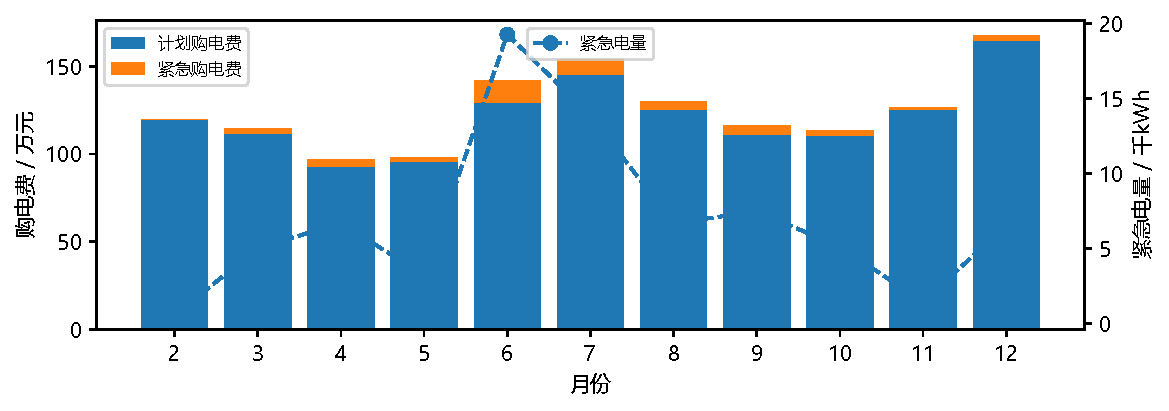
\includegraphics[width=0.86\textwidth]{figures/q2_month.pdf}
  \caption{月度购电费用构成与月度紧急购电量}
  \label{fig:q2_month}
\end{figure}

\begin{figure}[ht]
  \centering
  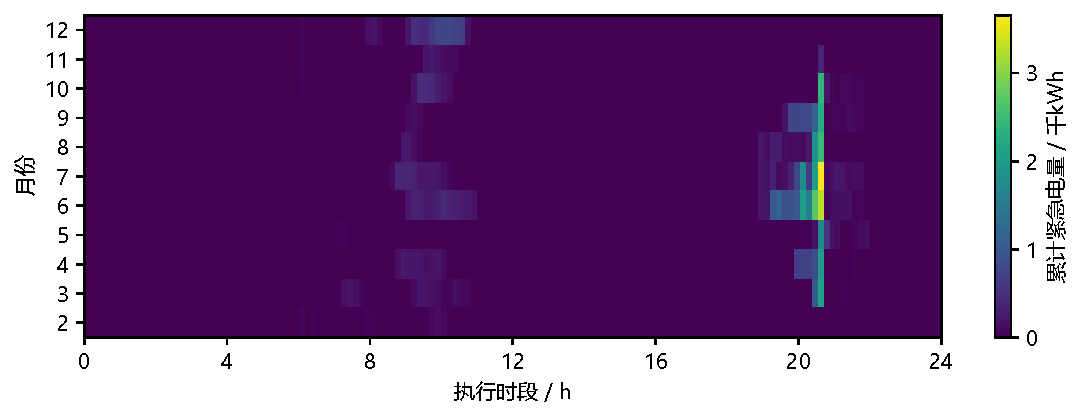
\includegraphics[width=0.94\textwidth]{figures/q2_heat.pdf}
  \caption{全年紧急购电量的月份—时刻分布热力图}
  \label{fig:q2_heat}
\end{figure}

\input{tables/问题二指定日期.tex}


\FloatBarrier
\section{问题三的分析、建模和求解}

\subsection{问题三的分析}

我们将附件3的四时刻预报细化至10分钟，并与基于当前决策时刻以前历史实测信息构造的统计预测融合，再用已完成时段的误差分位数构造净负荷经验分位数带。模型在日前计划基础上加入调整变量和偏差费用，于6:00、12:00、18:00按历史误差情景筛选是否调整。

\subsection{问题三的建模}
\subsubsection{数据预处理}

问题三在问题二的历史实测数据之外新增附件3的光伏功率预报。两类数据记录口径不同，我们先统一时间和功率单位，再进行融合。

第一步是预报数据的时间细化。附件3按0:00、6:00、12:00、18:00四个发布时刻分别给出未来24小时的逐小时光伏功率预报，而模型的时间步长为10分钟，故须作尺度细化。我们以发布时刻最近已完成时段的实测功率$v_0$为起点，将逐小时预报值作为节点作线性插值，得到10分钟粒度的预报曲线：
\begin{equation}\label{eq:src30}
    Y_{s,t}=\left[Y^{(h)}+\bigl(Y^{(h+1)}-Y^{(h)}\bigr)\theta\right]\Delta t,
 \quad\theta=\frac{u_t-h}{1\text{ h}},\quad h\le u_t<h+1,
\end{equation}
其中，$Y^{(h)}$为发行时刻之后第$h$小时的预报功率（kW），$Y^{(0)}=v_0$；$u_t$为目标时段结束时刻相对发行时刻的小时数，$Y_{s,t}$为插值后乘以$\Delta t$的时段电量（kWh）。未被该次预报覆盖的时段由历史预测补齐。

第二步是预报偏差的标定。将细化后的预报曲线与附件2的光伏实测序列逐时段作差，得到以发布时刻与小时编号为索引的偏差样本：
\begin{equation}\label{eq:src31}
    z_{s,t}^{(d)}=V_t^{(d)}-Y_{s,t}^{(d)},\qquad s\in\{0,1,2,3\},\quad t\ge36s
\end{equation}
其中，$s$为发布序号，对应时刻为$6s$时；$z_{s,t}^{(d)}$为第$d$天该次发布对第$t$时段的预报偏差（kWh）。我们按小时$h=\lfloor t/6\rfloor$汇总六个时段的误差样本。仅在有效时段已经完成后登记误差；官方产品的校正误差与最终融合净负荷误差分别保存，后者用于滚动筛选。

第三步是融合预报的构造。记历史统计预报为$\hat{V}_t^{\text{hist}}$（由式\eqref{eq:src14}的同时段基准加偏差修正给出），官方预报为$Y_t$，二者按权重$\omega_t$融合：
\begin{equation}\label{eq:src32}
    \hat V_t^{\mathrm{fus}}=\max\{0,\omega_t(Y_{s,t}+b^O_{s,h})+(1-\omega_t)\hat V_t^{\mathrm{hist}}\},\qquad
 \omega_t=\frac{\mathrm{MAE}_{H,s,h}}{\mathrm{MAE}_{O,s,h}+\mathrm{MAE}_{H,s,h}+10^{-9}}.
\end{equation}
其中，$b^O_{s,h}$为对应官方预报历史误差的小时中位数，两项MAE分别评价官方与历史预测。样本不足时日间权重取0.6；0--6时及19--24时权重取0.5、不作官方小时偏差校正。日间权重随已实现误差动态更新，各时段均保留原始光伏观测。

第四步是分位数带的构造。以同发布序号、同小时内六个时段的净负荷历史误差样本为基础，给出0.70与0.90两个分位数所对应的上下边界：
\begin{equation}\label{eq:src33}
    B_{t}^{\text{lo}}=\hat{N}_{t}+e_{t,0.70},\qquad B_{t}^{\text{hi}}=\hat{N}_{t}+e_{t,0.90}
\end{equation}
该分位数带用于第四种备选合同的方向约束。模型在6、12、18时根据当前已发布预报和已完成观测复核合同。

经上述处理，我们得到两类输入：日前滚动规划所需的预测序列，以及用于筛选合同的历史误差路径。



\paragraph{组合预测的估计机制与更新顺序}
历史光伏预测包含七日加权同时段均值与近28日中位数偏差两部分。前者保留日内出力形态并增加近期观测的权重，后者修正持续高估或低估。中位数是绝对偏差损失的最小化解：
\begin{equation}\label{eq:median_fit}
 b^* = \arg\min_b\sum_{e\in\mathcal R}|e-b|.
\end{equation}
官方预报的小时偏差采用相同估计准则。式\eqref{eq:src32}的组合权重使历史误差较小的预测源获得较大权重；每次权重更新均读取已经完成时段的误差档案。

对第$d$天，我们先用此前观测计算历史基准及校正量；在0时融合新发布预报并冻结日前预测，生成原计划；在6、12、18时更新未执行窗口并生成备选合同；当日观测完成后，将预测误差归入误差档案，跨日误差在次日相应时段完成后登记。各发布时点均先更新信息、再提交合同；实时执行只使用截至当前已实现的观测，满足滚动预测控制的时序约束\cite{parisio2014mpc}。

\subsubsection{问题三模型}

设第$d$天的四个预报发布时刻为0:00、6:00、12:00与18:00，其对应的时段编号依次为0、36、72与108。在第$s$次发布的时刻，调度中心可获取的信息集为
\begin{equation}\label{eq:src34}
    \mathcal{F}_{s}^{(d)}=\left\{\left(L_{t}^{(d)}\right)_{t<t_{s}},\ \left(V_{t}^{(d)}\right)_{t<t_{s}},\ \left(Y_{t}^{(s')}\right)_{s'\le s},\ \left(L_{t}^{(k)},V_{t}^{(k)}\right)_{k<d},\ p_{t}\right\}
\end{equation}

记第$d$天的计划购电量为$q_t$，生效购电量为$a_t$。为刻画调整行为，我们引入分解式
\begin{equation}\label{eq:src35}
    a_{t}=q_{t}+\Delta_{t}^{+}-\Delta_{t}^{-},\qquad \Delta_{t}^{+},\Delta_{t}^{-}\ge 0
\end{equation}
我们定义$\Delta_t^+=[a_t-q_t]^+$、$\Delta_t^-=[q_t-a_t]^+$，二者不同时为正。原计划在0时固定；后续调整不得修改已经执行的合同前缀：
\begin{equation}\label{eq:src36}
    a_t^{\mathrm{new}}=a_t^{\mathrm{old}},\qquad t<t_s
\end{equation}
为刻画合同的柔性程度，我们引入混合系数$\lambda\in\{0,0.5,1\}$，调整后的合同电量由当前生效合同与再优化解按比例混合而成：
\begin{equation}\label{eq:src37}
    a_{t}^{\lambda}=a_t^{\mathrm{old}}+\lambda\left(a_{t}^{\star}-a_t^{\mathrm{old}}\right),\qquad t\ge t_{s}
\end{equation}
其中，$a_t^{\star}$为在当前信息集下重新求解得到的理想购电量（kWh）。

第四条备选方案使用前节的分位数边界：若$q_t<B_t^{\mathrm{lo}}$，限制$a_t\ge q_t$；若$q_t>B_t^{\mathrm{hi}}$，限制$B_t^{\mathrm{hi}}\le a_t\le q_t$；其余样本充分的时段固定$a_t=q_t$。边界截为非负电量，样本不足时固定当前生效合同。在上述区间约束及储能约束下求解LP，得到分位数约束曲线。



题目给出的调整计价规则是分段的：上调部分按交易时刻电价的1.5倍采购；取消部分不再供电，但仍承担其原价50\%的违约成本，紧急购电则按5倍电价结算。据此，我们将单日总购电费用写为
\begin{equation}\label{eq:src38}
    \begin{aligned}
    C={}&\underbrace{\sum_{t\in\mathcal{T}}p_{t}\,q_{t}}_{\text{计划购电费}}
    +\underbrace{1.5\sum_{t\in\mathcal{T}}p_{t}\,\Delta_{t}^{+}}_{\text{新增采购费}}
    -\underbrace{0.5\sum_{t\in\mathcal{T}}p_{t}\,\Delta_{t}^{-}}_{\text{取消返还}}
    +\underbrace{5\sum_{t\in\mathcal{T}}p_{t}\,h_{t}}_{\text{紧急购电费}}
    \end{aligned}
\end{equation}
式\eqref{eq:src38}关于决策变量为线性函数。

\subsubsection{目标函数}

第$s$次决策时，未来时段的实际净负荷尚未揭示。主线性规划针对当前冻结的预测路径生成调整方案；历史误差路径构成的情景集用于方案筛选与风险检验，不改变主线性规划的目标函数：
\begin{equation}\label{eq:src39}
    \begin{aligned}
    \min\ F(a)={}&\sum_{i\in\mathcal H}\hat p_i a_i
    +0.5\sum_{i\in\mathcal D}\hat p_i z_i
    +5\sum_{i\in\mathcal H}\hat p_i h_i-0.45E_H,\\
    &z_i\ge |a_i-q_i|.
    \end{aligned}
\end{equation}
其中，$\mathcal H$为最长24小时窗口，$\mathcal D$为当前自然日尚未执行的合同格；次日尚未签约格只计正常采购费。末端价值不进入真实账单。我们先最小化完整$F$，再在$F\le F^*+10^{-6}$下最小化充放电总量；第四种备选方案不启用第二级。情景集$\mathcal{P}$由决策日之前若干完整日中同一发布时刻、同一时段区间的净负荷预报偏差序列构造，用于计算备选方案的情景费用并执行式\eqref{eq:src40}至式\eqref{eq:src42}的净增益筛选；情景费用平均值不进入主LP目标。


有限评价窗口可能使部分合同以消耗更多末端储电换取当前费用下降，因此对相对保持方案的末端储电短缺按机会成本扣价，构造净增益指标：
\begin{equation}\label{eq:src40}
    \left\{\begin{aligned}
    \hat{G}_{\varsigma}&=G_{\varsigma}-\kappa\,D_{\varsigma},\\[1mm]
    G_{\varsigma}&=C_{\varsigma}^{\text{keep}}-C_{\varsigma}^{\lambda},\\[1mm]
    D_{\varsigma}&=\left[E_{H}^{\text{keep}}-E_{H}^{\lambda}\right]^{+}
    \end{aligned}\right.
\end{equation}
$\kappa$的取值由紧急购电的机会成本决定：
\begin{equation}\label{eq:src41}
    \kappa=5\,\eta_{d}\,p_{\max}=5\times0.9\times1.3952=6.2784\ \text{元/kWh}
\end{equation}
其中，$p_{\max}=1.3952$元/kWh为附件1电价的最大值。这一取值按末端储电可替代的高价紧急采购作保守估值，其单位为元/电池内部kWh，仅用于备选方案的跨日储电价值比较。

基于净增益指标，调整的接受条件为
\begin{equation}\label{eq:src42}
    \dfrac{1}{\left|\mathcal{P}\right|}\sum_{\varsigma\in\mathcal{P}}\hat{G}_{\varsigma}>\varepsilon_{C},\qquad \varepsilon_{C}=5\ \text{元}.
\end{equation}
我们从满足式\eqref{eq:src42}的调整方案中取平均净增益最大的方案；若没有方案通过，则保持当前合同。各路径按问题二的实时规则运行至次日06:00，最多使用14条完整历史路径，不足7条时保持当前合同。

\subsubsection{约束条件}

第$s$次决策的备选合同须满足如下约束，其中功率平衡、储电量递推和储能边界分别对应式\eqref{eq:src43}至式\eqref{eq:src45}：
\begin{align}
    a_{t}+h_{t}+V_{t}+d_{t}&=L_{t}+c_{t}+w_{t},\qquad \forall t\in\mathcal{T}\label{eq:src43}\\
    E_{t+1}&=E_{t}+\eta_{c}\,c_{t}-\frac{d_{t}}{\eta_{d}},\qquad \forall t\in\mathcal{T}\label{eq:src44}\\
    E_{\min}&\le E_{t}\le E_{\max},\qquad 0\le c_{t},d_{t}\le \bar{Q},\qquad \forall t\in\mathcal{T}
\label{eq:src45}\end{align}
储电量边界同时施加于窗口终态$E_H$，即$E_{\min}\le E_H\le E_{\max}$，窗口初态固定为决策时刻已实现的储电量。规划使用当前预测，实际执行使用已实现的负载与光伏。


\textbf{我们建立以下基于线性规划与情景净增益的滚动优化模型：}
\begin{equation}\label{eq:src46}
    \begin{aligned}
    \min\quad &F(a)=\sum_{i\in\mathcal H}\hat p_i a_i+0.5\sum_{i\in\mathcal D}\hat p_i z_i+5\sum_{i\in\mathcal H}\hat p_i h_i-0.45E_H\\
    \mathrm{s.t.}\quad &a_t+h_t+V_t+d_t=L_t+c_t+w_t,\quad t\in\mathcal T,\\
    &E_{t+1}=E_t+\eta_c c_t-d_t/\eta_d,\quad E_{\min}\le E_t\le E_{\max},\\
    &a_t=q_t+\Delta_t^+-\Delta_t^-,\quad z_i\ge|a_i-q_i|,\\
    &\Delta_t^+,\Delta_t^-,c_t,d_t,h_t,w_t\ge0,\quad c_t,d_t\le\bar Q.
    \end{aligned}
\end{equation}
目标系数按完整$F$设置，情景筛选在模型求解后执行。算法参数如表\ref{tab:参数3}所示。

\Needspace{0.40\textheight}
\begin{longtable}{>{\centering\arraybackslash}p{0.1759\textwidth}>{\raggedright\arraybackslash}p{0.2932\textwidth}>{\centering\arraybackslash}p{0.1173\textwidth}>{\raggedright\arraybackslash}p{0.2736\textwidth}}
  \caption{问题三算法参数设置}
  \label{tab:参数3} \\
  \toprule
  参数名 & 参数含义 & 取值 & 选取依据 \\
  \midrule
  \endfirsthead
  \caption{问题三算法参数设置（续）} \\
  \toprule
  参数名 & 参数含义 & 取值 & 选取依据 \\
  \midrule
  \endhead
  \bottomrule
  \endfoot
  $\alpha$ & 日前保护分位数 & 0.8/0.7 & 0--6时/其余时段；取5日误差 \\
  $\lambda$ & 合同混合系数备选集合 & \{0, 0.5, 1\} & 半幅与完整两档调整 \\
  $\kappa$ & 终端储电量短缺惩罚系数（元/kWh） & 6.2784 & $5\eta_dp_{\max}$，式\eqref{eq:src41} \\
  $\varepsilon_C$ & 净增益均值门槛（元） & 5.0 & 排除预计微小收益 \\
  $r$ & 旧对照最坏情形预算（元） & 5.0 & 正式方案不启用该约束 \\
  $|\mathcal{P}|$ & 情景数（误差路径条数） & 7--14 & 不足7条保持当前合同 \\
  $\omega_t$ & 融合预报权重 & 随误差更新 & 冷启动0.6；特定夜间0.5 \\
  $5$ & 紧急购电价格倍数 & 5.0 & 题目给定 \\
\end{longtable}



记净负荷预测误差为$e_{s,t}^{(k)}=N_t^{(k)}-\hat N_{s,t}^{(k)}$，取决策日前已完成的同发布时刻路径，构造
\begin{equation}\label{eq:net_scenario}
 \widetilde N_{s,t}^{(d,\varsigma)}=\hat N_{s,t}^{(d)}+e_{s,t}^{(k_\varsigma)},
 \qquad k_\varsigma<d.
\end{equation}
每条路径保留连续时段误差，并对保持合同与调整方案采用相同初始状态和执行规则。

算法在每个调整时刻冻结信息、生成备选方案并进行历史路径筛选，选择平均净增益最大的合同后进入下一次滚动调整。

\subsection{求解结果}

\renewcommand{\arraystretch}{1.25}
\setlength{\LTpre}{6pt}
\setlength{\LTpost}{6pt}

我们采用Python调用SciPy/HiGHS线性规划求解器，基于附件2实测值与附件3预报，从2025年1月1日连续运行至年末，以1月形成历史预测与储电状态，统计2月至12月334天的费用。每天6、12、18时进行调整判定，共1002次机会；参数见表\ref{tab:参数3}。

\begin{longtable}{>{\centering\arraybackslash}p{0.2430\textwidth}>{\centering\arraybackslash}p{0.1870\textwidth}>{\centering\arraybackslash}p{0.2430\textwidth}>{\centering\arraybackslash}p{0.1870\textwidth}}
  \caption{问题三全年费用构成与运行指标}
  \label{tab:q3_sum} \\
  \toprule
  指标 & 数值 & 指标 & 数值 \\
  \midrule
  \endfirsthead
  \caption{问题三全年费用构成与运行指标（续）} \\
  \toprule
  指标 & 数值 & 指标 & 数值 \\
  \midrule
  \endhead
  \bottomrule
  \endfoot
  全年购电费（元） & 13298484.49 & 计划购电费用（元） & 12944853.84 \\
  新增采购费用（元） & 161738.79 & 取消返还金额（元） & 53888.71 \\
  紧急购电费用（元） & 245780.57 & 紧急购电量（kWh） & 42914.20 \\
  计划购电量（kWh） & 21231503.86 & 生效购电量（kWh） & 21135791.08 \\
  全年上调电量（kWh） & 111223.01 & 全年下调电量（kWh） & 206935.78 \\
  未消纳电量（kWh） & 2014393.07 & 年末储电量（kWh） & 2054.64 \\
  发起调整次数 & 265 & 保持当前合同次数 & 737 \\
  LP求解失败次数 & 0 & 核查异常次数 & 0 \\
\end{longtable}

\textbf{总费用为13298484.49元；1002次机会中调整265次，占26.45\%，紧急购电量为42914.20 kWh。}

\begin{figure}[ht]
  \centering
  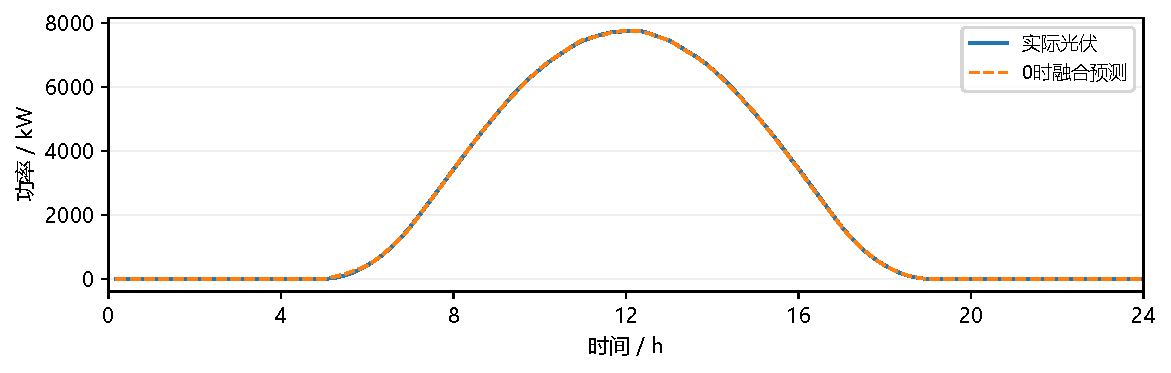
\includegraphics[width=0.86\textwidth]{figures/q3_forecast.pdf}
  \caption{光伏日前预测与实际出力的日内均值对比}
  \label{fig:q3_fc}
\end{figure}

\begin{figure}[ht]
  \centering
  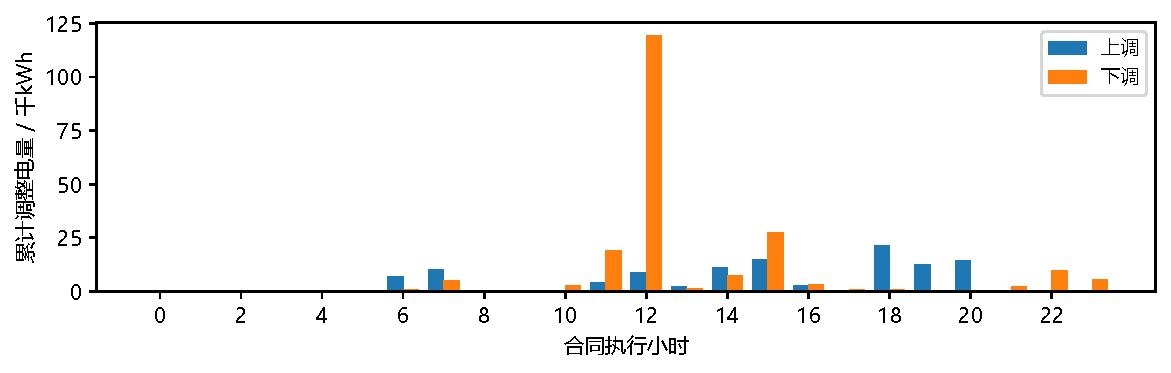
\includegraphics[width=0.86\textwidth]{figures/q3_adjust.pdf}
  \caption{各执行小时的全年上调与下调电量}
  \label{fig:q3_adj}
\end{figure}

\subsubsection{日前组合预测的时序回测}
我们采用滚动预测起点评价方法\cite{hyndman2021fpp}，以1月数据初始化误差档案，依次在2月1日至12月31日的每日0时预测随后144个时段。预测值提交后冻结，日终计算误差并更新档案。固定原模型参数重新运行预测模块，负载及融合光伏的逐时段输出均与正式轨迹一致。评价中始终用预测起点之前的观测更新估计量。

在48096个未来目标时段上，我们得到历史光伏预测与组合预测的MAE分别为150.18和127.90 kW，后者降低14.83\%；RMSE由306.25降至255.83 kW，降低16.46\%。组合预测的月度MAE范围为74.27至155.15 kW，月度误差随出力规模变化，因此同时以加权绝对百分比误差衡量相对预测精度，定义见模型检验部分。年度组合预测WAPE为5.38\%。

问题三较问题二的月度费用降幅为0.94\%至8.21\%。

\input{tables/问题三指定日期.tex}


\FloatBarrier
\section{问题四的分析、建模和求解}

\subsection{问题四的分析}

我们统计附件4的实时价格波动，并用目标日前的同日同时段价格及偏差中位数构造保守预测，并将问题二、问题三模型的电价系数替换为该预测价格，分别重解两类场景，再按实际价格结算并核查运行约束。



\subsection{问题四的建模}
\subsubsection{数据预处理}

问题四在问题二数据基础上加入附件4的实时电价序列。附件4按日、按10分钟记录价格，预处理先刻画价格特征，再构造可比的日前预测。

第一步是价格序列的对齐与统计。附件4的记录间隔同样为10分钟，与附件2的负载、光伏序列在时间上完全对齐，可直接按日、按时段组织为$p_t^{(d)}$。我们对其作统计刻画，得到全年实时电价的均值、标准差与变异系数：
\begin{equation}\label{eq:src47}
    \left\{\begin{aligned}
    \bar{p}&=\frac{1}{N}\sum_{d,t}p_{t}^{(d)}=0.7662,\\[1mm]
    \sigma_{p}&=\sqrt{\frac{1}{N}\sum_{d,t}\left(p_{t}^{(d)}-\bar{p}\right)^{2}}=0.3407,\\[1mm]
    \mathrm{CV}_{p}&=\frac{\sigma_{p}}{\bar{p}}=44.46\%
    \end{aligned}\right.
\end{equation}
其中，$N=365\times144$为全年样本总数。实时电价的最小值为0.0076元/kWh、最大值为1.7936元/kWh，峰谷比达236倍，而附件1的固定电价峰谷比仅3.76倍，说明实时电价的波动强度远高于固定电价。

第二步是价格不确定性度量。除全年的整体波动外，我们还需刻画电价在日内与逐日两个尺度上的波动强度：
\begin{equation}\label{eq:src48}
    \left\{\begin{aligned}
    \sigma_{\text{日内}}&=\frac{1}{365}\sum_{d}\mathrm{std}_{t}\left(p_{t}^{(d)}\right)=0.3229,\\[1mm]
    \sigma_{\text{逐日}}&=\mathrm{std}_{d}\left(\frac{1}{144}\sum_{t}p_{t}^{(d)}\right)=0.1036
    \end{aligned}\right.
\end{equation}
其中，$\sigma_{\text{日内}}=0.3229$元/kWh为365天日内电价标准差的均值，约为全年平均电价的42\%，说明日内价格差明显，储能可利用的价格差需要在效率与功率约束下判断；日均电价的取值范围为0.5378至0.9290元/kWh。这些指标描述实现价格的波动，不等同于预测误差或不可预测性。

第三步是价格预测的构造。与负载、光伏的预测同构，电价预测也采用“同时段基准＋偏差校正”的形式，且同样遵守因果性约束，即日前不使用当天未来实际价格；日内更新仅使用已完成时段的价格：
\begin{equation}\label{eq:src49}
    \hat{p}_{t}^{(d)}=\max\left\{p_{t}^{(d-7)}+\mathrm{median}_{k\in\mathcal K_d}\!\left(p_{t}^{(k)}-p_{t}^{(k-7)}\right),\ 10^{-4}\right\}
\end{equation}
其中，$p_t^{(d-7)}$为上周同日同时段的价格基准，$\mathcal K_d$为第$d$天之前、周同期数据已存在的最近最多$W=28$个已完成日。第二项为这些日期同一时段“周同比变化量”的中位数，起偏差校正作用；样本不足28日时使用已有样本，空集校正量取0。年初前7天以附件1电价作基准。下界$10^{-4}$用于避免价格为零时目标函数退化。式\eqref{eq:src49}的结构与式\eqref{eq:src18}一致，使得问题四可以复用问题二与问题三的求解流程。

经上述处理，我们得到实时价格的统计特征和日前预测序列，购电决策沿用问题二、问题三的储能与滚动调整框架。



\paragraph{季节性价格预测的统计解释}
式\eqref{eq:src49}以周周期季节性朴素预测为基准\cite{hyndman2021fpp}，并对最近最多28日同槽周同比变化作中位数校正。周周期项刻画同一星期位置的价格形态，中位数校正项刻画近期价格水平偏移，估计准则与式\eqref{eq:median_fit}一致。我们每天0时生成规划窗口的价格曲线，冻结当天24小时预测用于回测；日内仅在6、12、18时，以最近已完成时段的预测残差对当前价格曲线作衰减修正：
\begin{equation}\label{eq:price_update}
 \hat p_{t+j\mid t}=\max\{10^{-4},\hat p_{t+j}+\beta^j(p_t-\hat p_t)\},
 \qquad j\ge1,\quad\beta=0.90.
\end{equation}
其中$t$为最近已完成时段，$\beta$控制局部偏差的持续时间。日内校正与日前校正共享历史可用性约束，日前冻结值用于统一比较不同日期的预测误差。

\subsubsection{问题四模型}

本问前置参数包括价格误差样本窗口$W=28$天、情景数$|\mathcal P|=7$--$14$、日前保护分位数$\alpha=0.8/0.7$、价格下界$10^{-4}$元/kWh及紧急购电价格倍数5。


设第$d$天第$s$次决策的信息集为$\mathcal{F}_s^{(d)}$，则在问题四中该信息集除包含式\eqref{eq:src34}的各项外，还须包含截至当前时刻的价格观测与预测：
\begin{equation}\label{eq:src50}
    \mathcal{F}_{s}^{(d)}=\left\{\left(L_{t}^{(d)},V_{t}^{(d)}\right)_{t<t_{s}},\ \left(Y_{t}^{(s')}\right)_{s'\le s},\ \left(p_{t}^{(d')}\right)_{d'<d},\ \left(p_t^{(d)}\right)_{t<t_s},\ \hat{p}_{s,t}^{(d)},\ \left(L_{t}^{(k)},V_{t}^{(k)}\right)_{k<d}\right\}
\end{equation}
其中，$\left(p_t^{(d')}\right)_{d'<d}$为历史实时价格观测，$\hat{p}_t^{(d)}$为由式\eqref{eq:src49}给出的预测价格。与问题三相比，电价由已知输入变为当前预测值，决策还使用截至当时已实现的价格与当前储电状态；购电与储能安排随可用价格信息更新。

\subsubsection{目标函数}

为刻画预测价格与真实价格的偏离，我们定义价格预测误差：
\begin{equation}\label{eq:src51}
    \left\{\begin{aligned}
    \zeta_{t}^{(d)}&=\ln p_{t}^{(d)}-\ln\hat{p}_{t}^{(d)},\\[1mm]
    \mathbb{E}\left[\zeta_{t}^{(d)}\right]&=b_{t},\\[1mm]
    \mathrm{Var}\left[\zeta_{t}^{(d)}\right]&=s_{t}^{2}
    \end{aligned}\right.
\end{equation}
其中，$b_t$与$s_t$分别为对数价格误差的均值与标准差，可由最近$W$天的样本作描述统计；实际筛选直接采用已实现的历史误差路径，不假定其服从正态分布。采用对数形式的原因是价格恒为正，对数误差可在不引入非负约束的情况下保持价格的符号性质。

在价格不确定的条件下，若仅以预测价格下的费用最小为目标，实际价格高于预测时可能出现费用超支。问题四场景一沿用问题二的主模型，场景二沿用问题三的情景后验筛选：我们先按当前预测价格路径生成备选决策，再用历史价格误差路径计算平均净增益：
\begin{equation}\label{eq:src52}
 \min F(\hat p)\quad\longrightarrow\quad
 |\mathcal P|^{-1}\sum_{\varsigma\in\mathcal P}\hat G_{\varsigma}>5\ \text{元}.
\end{equation}
其中，$\mathcal P$由历史价格误差与同源净负荷误差共同构成，$\hat G$沿用问题三已计末端储电不足的净收益。无调整场景执行日前计划，时序回测给出实际费用和物理约束结果。


问题四分别求解合同不可调整与允许指定时刻调整的两类场景。

场景一（对应问题二）不含日内调整，取式\eqref{eq:src35}中的$\Delta_t^{+}=\Delta_t^{-}=0$，则生效购电量与计划购电量相等，费用函数退化为
\begin{equation}\label{eq:src53}
    \begin{aligned}
    C_{1}={}&\sum_{t\in\mathcal{T}}p_{t}^{(d)}\,q_{t}+5\sum_{t\in\mathcal{T}}p_{t}^{(d)}\,h_{t}
    \end{aligned}
\end{equation}
其中，$p_t^{(d)}$在计划阶段取预测价格$\hat{p}_t^{(d)}$、在结算阶段取真实价格$p_t^{(d)}$；价格不确定性由计划价与结算价的差异进入费用。

场景二（对应问题三）保留日内调整，费用函数仍为式\eqref{eq:src38}的四项结构，只是其中的价格由固定的$p_t$替换为逐日的$p_t^{(d)}$：
\begin{equation}\label{eq:src54}
    \begin{aligned}
    C_{2}={}&\sum_{t\in\mathcal{T}}p_{t}^{(d)}\,q_{t}
    +1.5\sum_{t\in\mathcal{T}}p_{t}^{(d)}\,\Delta_{t}^{+}
    -0.5\sum_{t\in\mathcal{T}}p_{t}^{(d)}\,\Delta_{t}^{-}
    +5\sum_{t\in\mathcal{T}}p_{t}^{(d)}\,h_{t}
    \end{aligned}
\end{equation}
三次调整决策的时刻与问题三一致，仍为6:00、12:00与18:00，问题四场景二沿用问题三式\eqref{eq:src40}至式\eqref{eq:src42}的净增益筛选；用于情景推演的价格由决策日前同发布时刻的历史对数价格误差路径构造：
\begin{equation}\label{eq:src55}
    \tilde{p}_{t}^{(d,\varsigma)}=\hat{p}_{t}^{(d)}\exp\left(\zeta_{t}^{(\varsigma)}\right),\qquad \zeta^{(\varsigma)}\in\mathcal{Z}_{p}^{(d)},\quad |\mathcal{Z}_{p}^{(d)}|\le14
\end{equation}
价格误差路径与对应净负荷误差路径按历史日期配对，情景数最多14条，至少保留7条才执行筛选。

\subsubsection{约束条件}

两类场景的约束条件与前三问一致，其中式\eqref{eq:src56}至式\eqref{eq:src58}分别对应功率平衡、储电量递推与储能运行边界：
\begin{align}
    a_{t}+h_{t}+V_{t}+d_{t}&=L_{t}+c_{t}+w_{t},\qquad \forall t\in\mathcal{T}\label{eq:src56}\\
    E_{t+1}&=E_{t}+\eta_{c}\,c_{t}-\frac{d_{t}}{\eta_{d}},\qquad \forall t\in\mathcal{T}\label{eq:src57}\\
    E_{\min}&\le E_{t}\le E_{\max},\qquad 0\le c_{t},d_{t}\le \bar{Q},\qquad \forall t\in\mathcal{T}
\label{eq:src58}\end{align}
储电量边界同时施加于窗口终态$E_H$，即$E_{\min}\le E_H\le E_{\max}$，窗口初态固定为决策时刻已实现的储电量。场景一固定$a_t=q_t$；场景二只允许在指定时刻修改未执行的合同，沿用问题三的净增益筛选。实际执行采用问题二逐时段规则。


\textbf{我们建立以下价格误差情景驱动的购电储能优化模型：}
\begin{equation}\label{eq:src60}
    \begin{aligned}
    \min\quad &F_j,\quad F_1=C_1-0.45E_H,\quad F_2=C_2-0.45E_H,\quad j\in\{1,2\},\\
    \mathrm{s.t.}\quad &a_t+h_t+V_t+d_t=L_t+c_t+w_t,\quad t\in\mathcal T,\\
    &E_{t+1}=E_t+\eta_c c_t-d_t/\eta_d,\quad E_{\min}\le E_t\le E_{\max},\\
    &0\le c_t,d_t\le\bar Q,\quad h_t,w_t\ge0,\\
    &a_t=q_t\ (j=1),\qquad a_t=q_t+\Delta_t^+-\Delta_t^-\ (j=2),\\
    &\Delta_t^+,\Delta_t^-\ge0.
    \end{aligned}
\end{equation}
主模型目标含末端储电价值$-0.45E_H$，电价系数取预测价格$\hat{p}_t^{(d)}$，参数见表\ref{tab:参数4}。

\Needspace{0.40\textheight}
\begin{longtable}{>{\centering\arraybackslash}p{0.1759\textwidth}>{\raggedright\arraybackslash}p{0.2932\textwidth}>{\centering\arraybackslash}p{0.1173\textwidth}>{\raggedright\arraybackslash}p{0.2736\textwidth}}
  \caption{问题四算法参数设置}
  \label{tab:参数4} \\
  \toprule
  参数名 & 参数含义 & 取值 & 选取依据 \\
  \midrule
  \endfirsthead
  \caption{问题四算法参数设置（续）} \\
  \toprule
  参数名 & 参数含义 & 取值 & 选取依据 \\
  \midrule
  \endhead
  \bottomrule
  \endfoot
  $\varepsilon_C$ & 净增益均值门槛（元） & 5.0 & 正式方案的接受条件 \\
  $r$ & 旧对照最坏损失预算（元） & 5.0 & 正式方案不启用该约束 \\
  $W$ & 价格误差样本窗口（日） & 28 & 与负载、光伏一致 \\
  $|\mathcal{P}|$ & 价格情景数 & 7--14 & 不足7条保持当前合同 \\
  $\alpha$ & 日前净负荷保护分位数 & 0.8/0.7 & 分别沿用对应问题配置 \\
  $5$ & 紧急购电价格倍数 & 5.0 & 题目给定 \\
  $10^{-4}$ & 价格下界（元/kWh） & $1\times10^{-4}$ & 避免目标退化 \\
\end{longtable}



我们对历史日期$k_\varsigma$同时提取净负荷误差$e_{s,t}^{(k_\varsigma)}$和对数价格误差$\zeta_{s,t}^{(k_\varsigma)}$，形成配对样本
\begin{equation}\label{eq:joint_scenario}
 \left(\widetilde N_{s,t}^{(d,\varsigma)},\widetilde p_{s,t}^{(d,\varsigma)}\right)
 =\left(\hat N_{s,t}^{(d)}+e_{s,t}^{(k_\varsigma)},
 \hat p_{s,t}^{(d)}\exp\zeta_{s,t}^{(k_\varsigma)}\right).
\end{equation}
同日期配对保留净负荷与价格偏差的共同变化，情景费用含紧急购电项与储能递推影响。

场景一按日前合同执行，场景二增加情景净增益筛选。

\subsection{求解结果}

\renewcommand{\arraystretch}{1.25}
\setlength{\LTpre}{6pt}
\setlength{\LTpost}{6pt}

我们采用Python调用SciPy/HiGHS线性规划求解器，基于上述模型利用附件4的实时电价、附件2的负载与光伏实测数据以及附件3的光伏预报，重新求解问题二与问题三所对应的两类场景，年度计算从1月1日连续运行至年末，以1月形成历史信息与储电状态，费用统一统计2025年2月1日至12月31日共334天。为便于对照，以下将“在固定电价下按问题二策略求解”记为方案一、“在波动电价下按问题二策略求解”记为方案二、“在固定电价下按问题三策略求解”记为方案三、“在波动电价下按问题三策略求解”记为方案四。

\Needspace{0.35\textheight}
\begin{longtable}{>{\centering\arraybackslash}p{0.1579\textwidth}>{\centering\arraybackslash}p{0.1393\textwidth}>{\centering\arraybackslash}p{0.1207\textwidth}>{\centering\arraybackslash}p{0.1207\textwidth}>{\centering\arraybackslash}p{0.1207\textwidth}>{\centering\arraybackslash}p{0.1207\textwidth}}
  \caption{四个方案的全年购电费与风险指标对比}
  \label{tab:q4_cmp} \\
  \toprule
  方案 & 全年购电费(元) & 紧急购电量(kWh) & 紧急购电费(元) & 未消纳电量(kWh) & 费用增幅(\%) \\
  \midrule
  \endfirsthead
  \caption{四个方案的全年购电费与风险指标对比（续）} \\
  \toprule
  方案 & 全年购电费(元) & 紧急购电量(kWh) & 紧急购电费(元) & 未消纳电量(kWh) & 费用增幅(\%) \\
  \midrule
  \endhead
  \bottomrule
  \endfoot
  方案一（固定电价，问题二） & 13790848.69 & 75858.03 & 468467.64 & 2687529.82 & — \\
  方案二（波动电价，问题二） & 14526595.92 & 75033.76 & 491939.63 & 2623658.96 & +5.34 \\
  方案三（固定电价，问题三） & 13298484.49 & 42914.20 & 245780.57 & 2014393.07 & — \\
  方案四（波动电价，问题三） & 14018361.30 & 41588.56 & 246697.18 & 1965903.51 & +5.41 \\
\end{longtable}

我们由表\ref{tab:q4_cmp}可知，电价由固定机制切换为实时波动机制后，方案二较方案一增加735747.23元，增幅为\textbf{5.34\%}；方案四较方案三增加719876.81元，增幅为\textbf{5.41\%}。在相同电价环境下进一步比较两类完整策略，可评价滚动机制的综合费用表现。在购电费上升的同时，方案二的紧急购电量、未消纳电量分别较方案一减少824.27 kWh与63870.86 kWh，方案四的紧急购电量、未消纳电量分别较方案三减少1325.65 kWh与48489.56 kWh。

\Needspace{0.35\textheight}
\begin{longtable}{>{\centering\arraybackslash}p{0.1179\textwidth}>{\centering\arraybackslash}p{0.1451\textwidth}>{\centering\arraybackslash}p{0.1451\textwidth}>{\centering\arraybackslash}p{0.1270\textwidth}>{\centering\arraybackslash}p{0.1360\textwidth}>{\centering\arraybackslash}p{0.1088\textwidth}}
  \caption{波动电价下指定日期的购电与紧急购电结果}
  \label{tab:q4_day} \\
  \toprule
  日期 & 计划购电量 & 生效购电量 & 紧急购电量 & 方案 & 日购电费 \\
   & (kWh) & (kWh) & (kWh) & — & (元) \\
  \midrule
  \endfirsthead
  \caption{波动电价下指定日期的购电与紧急购电结果（续）} \\
  \toprule
  日期 & 计划购电量 & 生效购电量 & 紧急购电量 & 方案 & 日购电费 \\
   & (kWh) & (kWh) & (kWh) & — & (元) \\
  \midrule
  \endhead
  \bottomrule
  \endfoot
  2025-03-20 & 64505.11 & 64505.11 & 86.51 & 方案二 & 41921.38 \\
  2025-06-21 & 42284.43 & 42284.43 & 0.00 & 方案二 & 20377.80 \\
  2025-09-23 & 70341.18 & 70341.18 & 1.08 & 方案二 & 46368.53 \\
  2025-12-21 & 94463.38 & 94463.38 & 16.04 & 方案二 & 72005.59 \\
  2025-03-20 & 64098.58 & 62700.51 & 270.74 & 方案四 & 42686.63 \\
  2025-06-21 & 42171.14 & 42171.14 & 0.00 & 方案四 & 20175.42 \\
  2025-09-23 & 69677.93 & 69677.93 & 1.08 & 方案四 & 45618.55 \\
  2025-12-21 & 94107.16 & 94107.16 & 33.05 & 方案四 & 71402.26 \\
\end{longtable}

我们由表\ref{tab:q4_day}可知，四个指定日期的购电费差异较大：12月21日的日购电费为72005.59元与71402.26元，约为6月21日的3.5倍。方案四在6月21日、9月23日和12月21日分别比方案二节省202.38元、749.98元和603.33元，但3月20日多支出765.25元。3月20日生效合同较原计划下调1398.07 kWh，且发生270.74 kWh紧急购电；其余三个指定日未调整合同。

\begin{figure}[ht]
  \centering
  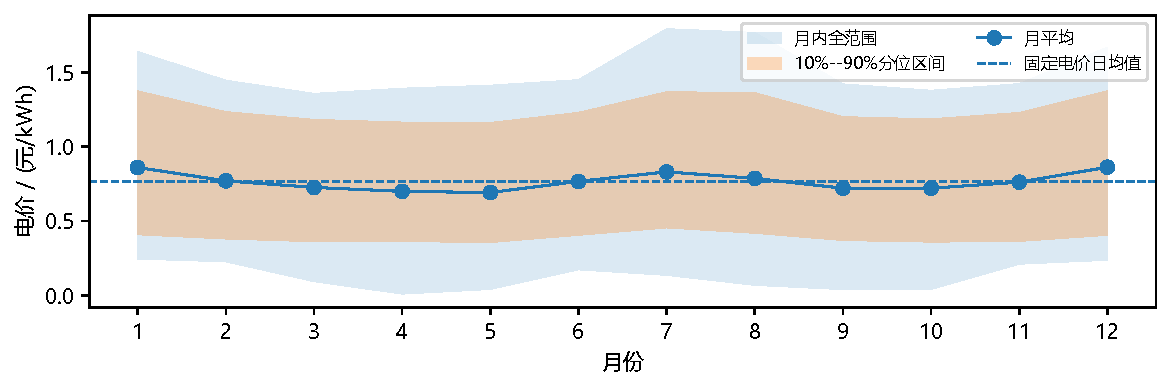
\includegraphics[width=0.86\textwidth]{figures/q4_price.pdf}
  \caption{全年电价的月度范围、分位区间与固定价日均值}
  \label{fig:q4_price}
\par\smallskip
\begin{minipage}{\textwidth}\small
图\ref{fig:q4_price}显示，实时电价的月度取值范围与分位区间存在明显差异，月内价格离散程度随月份变化。预测价格通过目标函数系数影响储能的充放电时序。
\end{minipage}
\end{figure}

% 指定日调度图与表格信息重复，正文保留价格波动、储能包络和风险图。

\begin{figure}[ht]
  \centering
  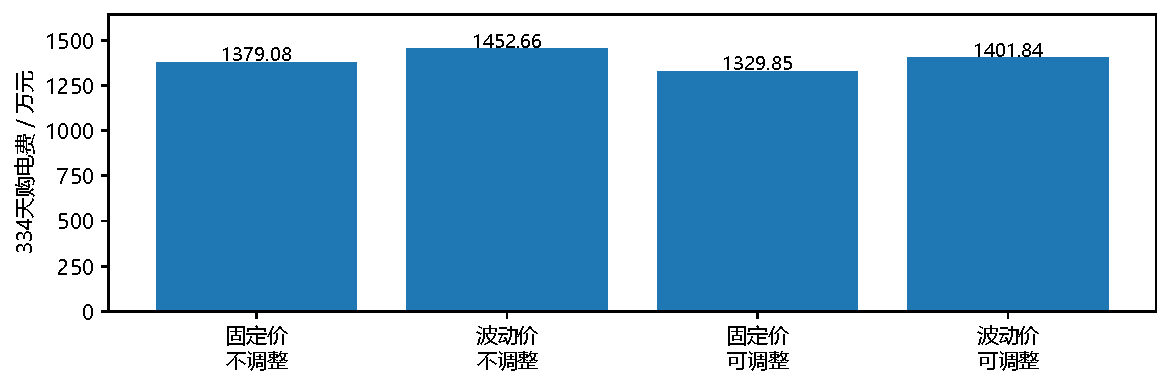
\includegraphics[width=0.86\textwidth]{figures/q4_cost.pdf}
  \caption{四个方案在334天评价区间的购电费对比}
  \label{fig:q4_cmp}
\par\smallskip
\begin{minipage}{\textwidth}\small
图\ref{fig:q4_cmp}显示，滚动调整方案的全年费用低于对应的日前方案，在固定电价和波动电价环境下分别节省\textbf{3.57\%}和\textbf{3.50\%}。
\end{minipage}
\end{figure}

\begin{figure}[ht]
  \centering
  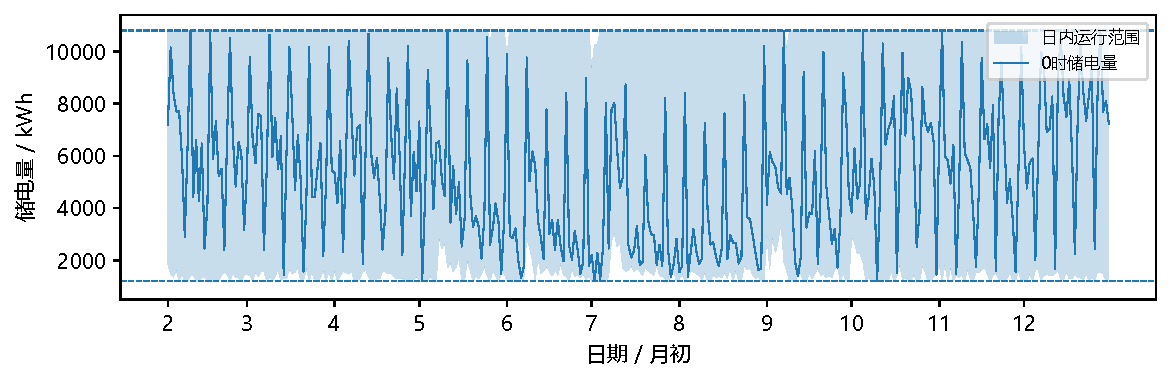
\includegraphics[width=0.84\textwidth]{figures/q4_soc.pdf}
  \caption{问题四跨日储能状态运行包络}
  \label{fig:q4_soc}
\par\smallskip
\begin{minipage}{\textwidth}\small
图\ref{fig:q4_soc}显示，储能状态始终处于1200至10800 kWh运行区间，各日储电量包络随供需和价格输入变化。
\end{minipage}
\end{figure}

\textbf{在波动电价下，正式可调整完整方案较不可调整完整方案节省508234.62元，节费3.50\%。}

\subsubsection{价格预测精度与跨月费用稳定性}
我们对问题四执行与问题三相同的逐日滚动起点回测。每日0时冻结未来24小时的价格预测，以附件4实现价格评价，得到MAE为0.04803元/kWh、RMSE为0.06570元/kWh、$R^2=0.9618$、WAPE为6.34\%。月度MAE介于0.03883与0.05917元/kWh之间。

为辨别偏差校正的作用，我们增加周同期季节性朴素预测作为基准，其MAE为0.04715元/kWh、RMSE为0.06535元/kWh。两种方法精度接近，周同期基准在本年度平均误差上略优。

我们将预测性能与运行性能分开统计，波动电价下完整滚动方案较对应日前方案的11个月费用均下降，月度降幅为1.19\%至8.51\%。这些月度差额反映完整策略在本年度实际价格与供需条件下的费用表现。


\FloatBarrier

\section{模型检验与分析}

模型检验分别考察预测误差、参数响应、组件作用、运行约束、分月费用及未来误差情景。费用均按实际生效合同、紧急购电量和实现价格结算。

\subsection{误差分析}

我们对2025年2月1日至12月31日334天的每日0时预测进行评价，共48096个10分钟时段，并采用$R^2$、RMSE、MAE和MAPE衡量误差\cite{hyndman2006another}；光伏MAPE只取实际功率大于50 kW的24207个时段，其余指标取全时段，结果见表\ref{tab:error}。

\Needspace{0.25\textheight}
\begin{longtable}{lrrrr}
\caption{日前预测误差}\label{tab:error}\\
\toprule 预测对象 & $R^2$ & RMSE/kW & MAE/kW & MAPE/\%\\
\midrule\endfirsthead
\caption{日前预测误差（续）}\\
\toprule 预测对象 & $R^2$ & RMSE/kW & MAE/kW & MAPE/\%\\
\midrule\endhead\bottomrule\endfoot
负载预测 & 0.9696 & 245.42 & 181.45 & 4.24\\
历史光伏预测 & 0.9896 & 306.25 & 150.18 & 6.95\\
融合光伏预测 & 0.9927 & 255.83 & 127.90 & 6.51\\
\end{longtable}

融合光伏预测的MAE较历史预测降低14.83\%，RMSE降低16.46\%。

\subsection{参数敏感性与价格尺度检验}

我们先检验问题一中价格变化的解析关系。全部电价同乘正系数$\rho$时，可行域及最优方案集合不变，$F^*(\rho p)=\rho F^*(p)$。电价整体降低或提高10\%后，典型日费用分别为31614.25元、38639.64元，变化率同为$\mp10\%$。

\Needspace{0.20\textheight}
我们在年度敏感性试验中固定数据、设备容量和功率边界，每次改变一个参数。可调整组沿用含最坏损失限制的实验对照$F$，不可调整组以问题二、四的对应正式方案为对照。两种电价下分别考察保护分位数$\alpha$、规划末端价值$\nu$、效率$\eta_c=\eta_d=\eta$、日前展望$H$及历史情景损失预算$r$，取值与费用响应见图\ref{fig:unified_sensitivity}。可调整组在0--6时取$\alpha$，其余时段取$\alpha-0.10$；不可调整组全天取同一$\alpha$。各曲线以对应对照费用$C_0$计算$(C-C_0)/C_0\times100\%$。

\begin{figure}[tbp]
\centering
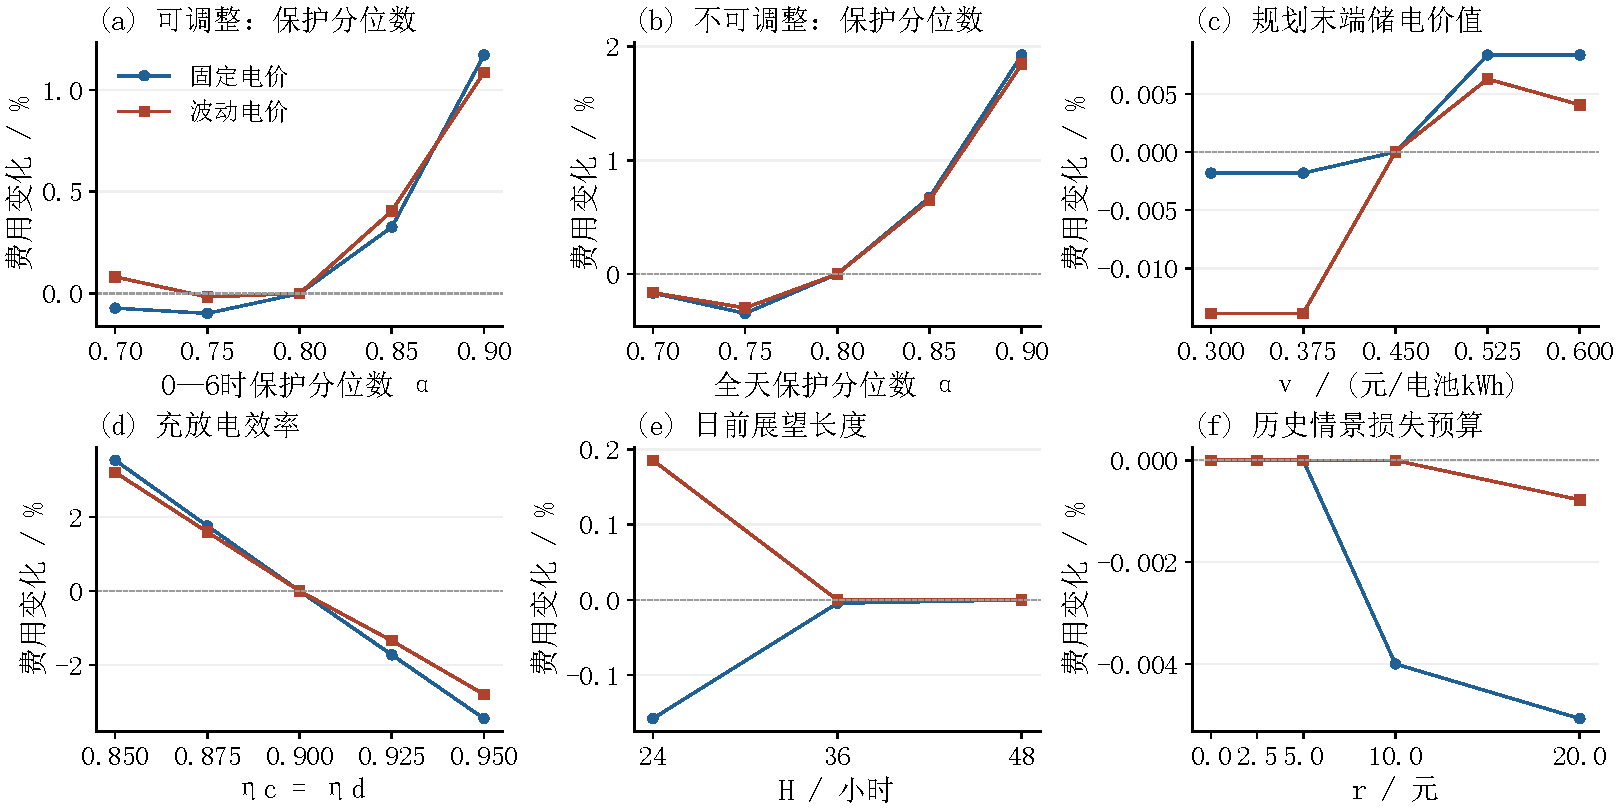
\includegraphics[width=\textwidth]{figures/统一参数敏感性.pdf}
\caption{参数变化下相对实验对照的评价期费用响应}
\label{fig:unified_sensitivity}
\end{figure}

在所设扰动范围内，效率变化引起的费用响应最大。$\eta$由0.85变为0.95时，固定电价费用相对对照$F$的变化由$+3.536\%$降至$-3.451\%$，波动电价由$+3.210\%$降至$-2.797\%$。这里改变的是单向充、放电效率，往返效率为$\eta^2$；调度与执行采用相同效率，式\eqref{eq:src41}的扣价随$\eta_d$变化。该试验表示对照配置下设备效率变化的后果，题目给定的0.90仍用于正式结果。

保护分位数在0.70至0.90内变化时，可调整方案的费用变幅为固定电价$-0.098\%$至$+1.172\%$、波动电价$-0.017\%$至$+1.086\%$；不可调整方案分别为$-0.347\%$至$+1.928\%$、$-0.299\%$至$+1.847\%$。提高保护量会同时改变正常购电和缺口补购，两类费用的平衡使响应并非处处单调。

在所取网格内，$\nu$的费用变幅绝对值不超过0.014\%，$r$不超过0.0051\%。$H$只改变日前展望，日内候选仍按最长24小时生成，情景评价仍延续至次日06:00；36小时与48小时的费用差仅为固定电价$-604.28$元、波动电价$-21.63$元。将预算$r$从5元调至20元引起的变化很小。

综上，模型在电价尺度、保护分位数、末端价值和预测展望等参数变化下均保持稳定的费用响应，说明所构建的参数体系具有良好的协调性，能够支持不同购电环境下的储能优化决策。

\subsection{年度策略局部消融检验}

为分辨各组件的作用，我们在两种电价下均使用相同负载、光伏及初始储电量6000 kWh，从1月1日连续运行365日；1月形成历史信息与储电状态，费用统一统计2--12月334日，并完成66组不同配置的消融与参数试验，重复的对照点复用同一结果。含最坏损失限制的对照$F$在固定、波动电价下的费用分别为13370019.70元和14078164.36元。正式可调整方案对应表\ref{tab:ablation}中“取消最坏损失限制”组，费用分别为13298484.49元和14018361.30元。

简单参照方案仅用历史预测，并同时取消日内调整、日前保护和规划末端价值。其余组相对$F$一次改变一项：仅0时预报组仍可在6、12、18时调整；取消日前保护组保留分位数约束候选；取消调整组保持$F$的预测和分位排程；$\nu$与$\kappa$分别取消；最坏损失组仅取消$\min_{\varsigma}\hat G_{\varsigma}\ge-r$，保留四个候选、相同历史路径及净增益均值条件。

\begingroup
\setlength{\tabcolsep}{6pt}
\Needspace{0.35\textheight}
\begin{longtable}{p{0.245\textwidth}rrrr}
\caption{组件变化相对含最坏损失限制对照$F$的费用与紧急购电量差}\label{tab:ablation}\\
\toprule
配置变化 & \multicolumn{2}{c}{费用差/元} & \multicolumn{2}{c}{紧急购电量差/kWh}\\
 & 固定电价 & 波动电价 & 固定电价 & 波动电价\\
\midrule\endfirsthead
\caption{组件变化相对含最坏损失限制对照$F$的费用与紧急购电量差（续）}\\
\toprule 配置变化 & \multicolumn{2}{c}{费用差/元} & \multicolumn{2}{c}{紧急购电量差/kWh}\\
 & 固定电价 & 波动电价 & 固定电价 & 波动电价\\
\midrule\endhead\bottomrule\endfoot
简单参照方案 & +1935181.49 & +2008272.62 & +458476.04 & +472222.26 \\
仅用0时光伏预报 & +3487.75 & +2951.83 & -930.55 & -1776.82 \\
取消日前保护量 & +268732.48 & +311355.36 & +113103.24 & +128400.37 \\
取消末端价值$\nu$ & -243.41 & -1954.81 & +40.98 & +8.82 \\
取消短缺扣价$\kappa$ & -14113.61 & -4817.05 & +191.94 & +1456.37 \\
取消最坏损失限制（正式） & -71535.21 & -59803.06 & -13861.25 & -12778.28 \\
取消日内合同调整 & +233906.53 & +269524.65 & +48720.06 & +50643.75 \\
仅用发布光伏预报 & +238475.28 & +277803.50 & +2638.32 & +5871.00 \\
\end{longtable}
\endgroup


相对$F$取消日前保护后，固定、波动电价费用分别增加2.01\%和2.21\%；光伏仅用发布预报、取消与历史预测的组合后，分别增加1.78\%和1.97\%。保持预测和保护配置，恢复$F$的日内合同调整，可使相应无调整方案的费用降低1.72\%和1.88\%。简单参照方案的费用增幅为14.47\%和14.27\%。

日内更新光伏预报后，6、12、18时各自未来6小时的合并MAE由158.13降至107.74 kW，降幅31.86\%，但费用只减少3487.75元和2951.83元，紧急电量也未同步减少。对同日费用差以7日连续移动块重采样10000次\cite{kunsch1989}，平均日差的95\%区间分别为$[-44.37,57.27]$元和$[-58.39,63.41]$元，均包含零。

末端价值的作用需结合评价边界考察。相对$F$取消$\nu$后，账单分别减少243.41元和1954.81元；另以统一参考价0.45元/电池kWh计算$C_{\rm ref}=C-0.45(E_{\text{末}}-E_{\text{初}})$，两组相对$F$仅差$+78.24$元和$-12.49$元。相对$F$取消$\kappa$后费用下降，但紧急购电量增加，调整次数由65、77次增至296、261次；两组平均日费用差区间分别为$[-67.95,-16.14]$元和$[-35.52,13.65]$元。短缺扣价在含最坏损失限制的配置下减少了合同变动；固定电价下有费用代价，波动电价下费用差方向尚不稳定。

取消最坏情景限制后，固定、波动电价费用分别减少71535.21元和59803.06元，11个月费用均下降；日费用与日紧急电量的最大值及95\%分位数也均下降。相应平均日费用差的95\%区间为$[-303.52,-130.51]$元、$[-274.80,-97.25]$元。

波动电价下，取消周同期偏差校正后，日前电价MAE由0.04803降至0.04715元/kWh；不可调整方案费用减少3288.75元，含最坏损失限制的可调整组相对$F$增加7980.31元。两者平均日差区间分别为$[-31.06,10.57]$元和$[-20.53,87.38]$元。

综合消融结果，净负荷保护、组合预测和日内合同调整共同改善了购电费用与紧急购电控制效果，完整模型在固定电价和波动电价场景下均取得稳定的综合收益，体现了各模块协同集成的优势。

\subsection{滚动预测起点与分月稳定性检验}
对每个预测起点$d$，我们仅使用该起点预测的未来一天进行误差统计，并将48096个10分钟目标时段按月份分组，定义
\begin{equation}\label{eq:validation_metrics}
\begin{aligned}
\mathrm{MAE}&=\frac1n\sum_i|y_i-\hat y_i|,\qquad
\mathrm{RMSE}=\sqrt{\frac1n\sum_i(y_i-\hat y_i)^2},\\
\mathrm{WAPE}&=\frac{\sum_i|y_i-\hat y_i|}{\sum_i|y_i|}\times100\%,\qquad
S_m=\frac{C_m^{\mathrm{base}}-C_m^{\mathrm{roll}}}{C_m^{\mathrm{base}}}\times100\%.
\end{aligned}
\end{equation}
其中$n$为评价时段数，$S_m$为第$m$月正式可调整方案相对对应日前方案的费用节省率。WAPE采用全样本实际值总量作分母，适合包含零出力时段的光伏序列。模型参数固定为正式配置，滚动更新的对象为历史误差及预测校正量。

\Needspace{0.35\textheight}
\begin{longtable}{rrrrrr}
\caption{分月预测误差与正式方案费用节省率}\label{tab:monthly_stability}\\
\toprule 月份 & 时段数 & 光伏MAE/kW & 电价MAE/(元/kWh) & 固定价$S_m$/\% & 波动价$S_m$/\%\\\midrule\endfirsthead
\caption{分月预测误差与正式方案费用节省率（续）}\\\toprule 月份 & 时段数 & 光伏MAE/kW & 电价MAE/(元/kWh) & 固定价$S_m$/\% & 波动价$S_m$/\%\\\midrule\endhead\bottomrule\endfoot
2 & 4032 & 99.59 & 0.04703 & 1.54 & 1.48\\
3 & 4464 & 128.04 & 0.04250 & 3.45 & 3.40\\
4 & 4320 & 155.15 & 0.04331 & 6.63 & 6.26\\
5 & 4464 & 145.25 & 0.04690 & 4.00 & 3.45\\
6 & 4320 & 143.50 & 0.05406 & 8.21 & 8.51\\
7 & 4464 & 154.09 & 0.05690 & 2.69 & 2.90\\
8 & 4464 & 154.21 & 0.04807 & 4.00 & 3.35\\
9 & 4320 & 134.08 & 0.05917 & 5.21 & 4.89\\
10 & 4464 & 137.59 & 0.04294 & 2.29 & 2.10\\
11 & 4320 & 78.41 & 0.03883 & 0.94 & 1.19\\
12 & 4464 & 74.27 & 0.04869 & 1.35 & 1.85\\

\end{longtable}
两类正式可调整方案在11个月的费用均低于对应日前方案，6月降幅最大，分别为8.21\%和8.51\%；11月最小，分别为0.94\%和1.19\%。


\section{模型评价与推广}
\subsection{模型优势}
我们在四问中采用相同的供需平衡和储电量递推关系，并根据可用预报、合同调整条件与电价描述不同购电任务；储能在有余电时充电、存在缺口时放电，从而明确计划量、补购量和费用之间的关系。

在含最坏损失限制的实验对照下，我们的消融结果支持净负荷保护、光伏组合预测和日内合同调整的作用。去掉日前保护后，两种电价下的费用分别增加2.01\%和2.21\%；去掉光伏组合后分别增加1.78\%和1.97\%。保持该对照的预测与保护安排时，允许合同调整分别减少23.39万元和26.95万元费用。

\subsection{适用条件与局限}
我们在正式方案中保留净增益均值门槛并取消最坏情景损失限制。相对含该限制的对照，固定与波动电价下的费用分别减少7.15万元和5.98万元，紧急购电量也降低，日费用与紧急电量的最大值及95\%分位数均下降。

2025年数据已参与此前配置选择，本次消融与敏感性分析属于同一年度的回顾性比较。模型的适用前提是近期误差仍有代表性、紧急购电能够保障供电、储能效率近似恒定；跨年度效果需用新增数据检验。

\subsection{模型改进与推广}
在含最坏损失限制的对照及所设扰动范围内，我们发现设备效率变化引起的费用变化最大：单向充放电效率由0.90降至0.85时，固定与波动电价下的费用分别增加3.54\%和3.21\%。推广时，应先根据设备实测数据估计效率随储电状态、充放电功率的变化，再加入循环寿命成本、功率爬坡和联络线容量限制。

针对风险限制的保守代价，我们可用新增年度数据比较不同历史误差窗口与损失预算下的实际费用、紧急购电和不利日期，选择与供电要求相适应的调整规则；气温、节假日等信息也可用于预测，并同时检验预测误差和购电费用。

% 参考文献沿用正文行距。
{\renewcommand{\baselinestretch}{1.15}\normalsize
\printbibliography[title={参考文献}]
}
\renewcommand{\baselinestretch}{1.22}\normalsize
\end{document}
